%%%%%%%%%%%%%%%%%%%%%%%%%%%%%%%%%%%%%%%%%%%%%%%%%%%%%%%%%%%%%%%%%%%%%%
% LaTeX Template: Beamer arrows
%
% Source: http://www.texample.net/
% Feel free to distribute this template, but please keep the
% referal to TeXample.net.
% Date: Nov 2006
% 
%%%%%%%%%%%%%%%%%%%%%%%%%%%%%%%%%%%%%%%%%%%%%%%%%%%%%%%%%%%%%%%%%%%%%%
% How to use writeLaTeX: 
%
% You edit the source code here on the left, and the preview on the
% right shows you the result within a few seconds.
%
% Bookmark this page and share the URL with your co-authors. They can
% edit at the same time!
%
% You can upload figures, bibliographies, custom classes and
% styles using the files menu.
%
% If you're new to LaTeX, the wikibook is a great place to start:
% http://en.wikibooks.org/wiki/LaTeX
%
%%%%%%%%%%%%%%%%%%%%%%%%%%%%%%%%%%%%%%%%%%%%%%%%%%%%%%%%%%%%%%%%%%%%%%

\documentclass[usenames,dvipsnames]{beamer} %
\usetheme{Madrid}
\usecolortheme{beaver}
\usepackage[latin1]{inputenc}
\usefonttheme{professionalfonts}
\usepackage{pifont}
\usepackage{tikz}
\usepackage{amsmath,amsfonts,amssymb}
\usepackage{verbatim}
\usepackage{hyperref}
\usepackage{subfigure}

\usepackage{xcolor}
\usepackage{media9}
\usepackage{animate}
\usepackage{booktabs}

\usepackage{color}
\usepackage{listings}

\definecolor{deepblue}{rgb}{0,0,0.5}
\definecolor{deepred}{rgb}{0.6,0,0}
\definecolor{deepgreen}{rgb}{0,0.5,0}

\DeclareMathOperator*{\argmax}{arg\,max}
\DeclareMathOperator*{\argmin}{arg\,min}

\usetikzlibrary{arrows,shapes}

%\beamerdefaultoverlayspecification{<+->}

\setbeamercolor{itemize item}{fg=red}
\setbeamercolor{itemize subitem}{fg=BrickRed}
\setbeamercolor{itemize subsubitem}{fg=black}

\setbeamertemplate{itemize item}[square]
\setbeamertemplate{itemize subitem}[circle]
\setbeamertemplate{itemize subsubitem}[triangle]

\setbeamertemplate{caption}[numbered]

\newcommand\bred[1]{\textcolor{red}{\textit{#1}}}
\newcommand\bblue[1]{\textcolor{blue}{\textit{#1}}}

\newcommand\vari[1]{\textcolor{BrickRed}{\texttt{#1}}}
\newcommand\defi[1]{\textcolor{NavyBlue}{\textit{#1}}}


\renewcommand{\figurename}{Figura}
\newcommand{\matr}[1]{\mathbf{#1}}

\author{MSc. Diego Porres}
\title{Elements of Machine Learning}
\subtitle{Introducci\'on}
\institute[UFM]{
\includegraphics[height=0.73cm, width=3.3cm]{images/LogotipoUFM_interna.png}}
\date{Enero 2019}


\begin{document}

\frame{\titlepage}

\begin{comment}
:Title: Beamer arrows
:Tags: Remember picture, Beamer, Physics & chemistry, Overlays
:Use page: 3

With PGF/TikZ version 1.09 and later, it is possible to draw paths between nodes across
different pictures. This is a useful feature for presentations with the
Beamer package. In this example I've combined the new PGF/TikZ's overlay feature
with Beamer overlays. Download the PDF version to see the result.

**Note.** This only works with PDFTeX, and you have to run PDFTeX twice.

| Author: Kjell Magne Fauske

\end{comment}


% For every picture that defines or uses external nodes, you'll have to
% apply the 'remember picture' style. To avoid some typing, we'll apply
% the style to all pictures.
\tikzstyle{every picture}+=[remember picture]

% By default all math in TikZ nodes are set in inline mode. Change this to
% displaystyle so that we don't get small fractions.
\everymath{\displaystyle}

\begin{frame}
    \begin{center}
	Some of the figures in this presentation are taken from \textit{An Introduction to Statistical Learning, with applications in R}  (Springer, 2013) with permission from the authors: G. James, D. Witten,  T. Hastie and R. Tibshirani
\end{center}
\end{frame}

\begin{frame}{Introducci\'on}

\begin{itemize}
    \item Acerca de m\'i:
    \begin{itemize}
        \item Licenciatura en F\'isica, UVG, Guatemala
        \item MSc. in Mathematical Engineering, Universidad de L\char`\'Aquila, Italia
        \item Master of Mathematics and Interactions, Universidad Nice-Sophia Antipolis, Francia
        \begin{itemize}
            \item Pasant\'ia en el Centre de Visi\'o per Computador, Barcelona, Espa\~na
            \item \small[Deep\small] Reinforcement Learning for Self-Driving Cars
        \end{itemize}
        \item Aplicaciones de drones a la agricultura de precisi\'on.
        \item ?`?
    \end{itemize}
\end{itemize}

\end{frame}

\begin{frame}{Pasant\'ia en el CVC - MsPacman}
%\begin{center}
%    \animategraphics[loop,width=0.75\linewidth]{15}{mspacman/mspacman-}{0}{127}
%\end{center}

\begin{figure}
	\centering
	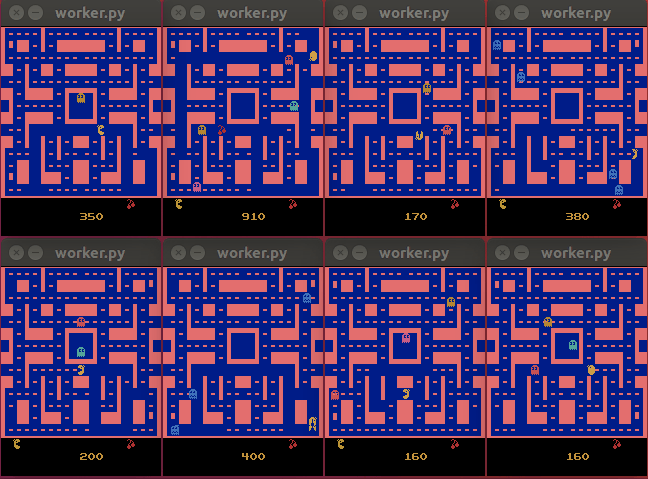
\includegraphics[width=0.70\textwidth]{mspacman/mspacman-0.png}
\end{figure}

\end{frame}

\begin{frame}{Pasant\'ia en el CVC - DuskDrive}
%    \begin{center}
%        \animategraphics[loop, width=0.75\textwidth]{8}{dusk/dusk-}{0}{80}
%    \end{center}
\begin{figure}
	\centering
	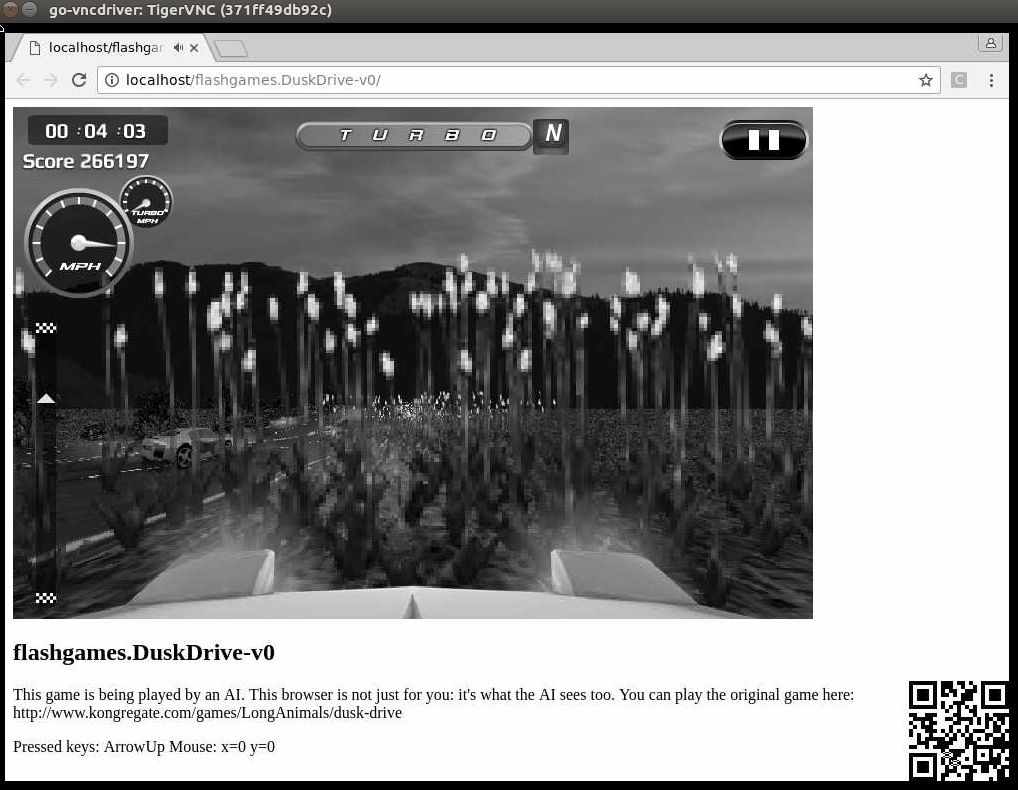
\includegraphics[width=0.70\textwidth]{dusk/dusk-0.png}
\end{figure}

\end{frame}

\begin{frame}{NeurIPS 2018: \textit{Latent Fabrics}}
\begin{figure}
	\centering
	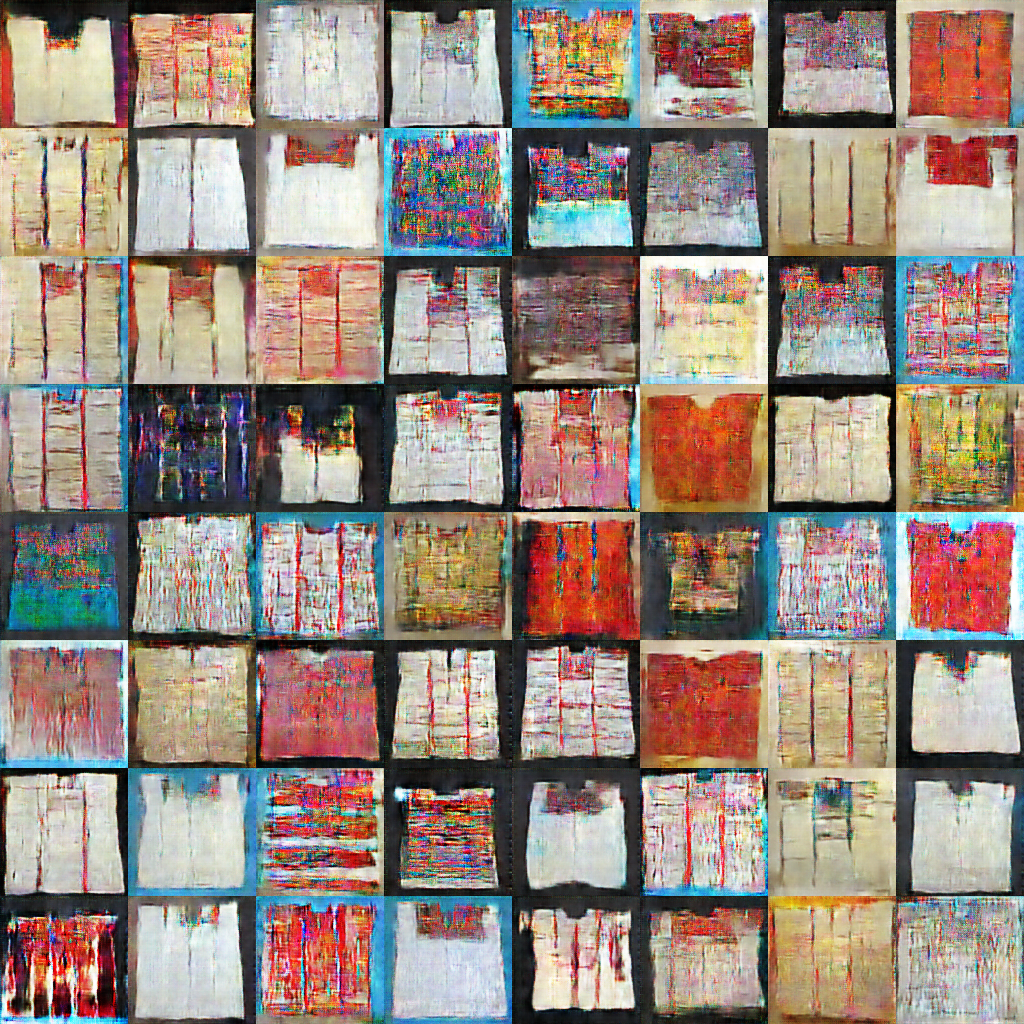
\includegraphics[width=0.4\textwidth]{latent/t-49.png}
\end{figure}

    \begin{center}
%        \animategraphics[loop, width=0.50\textwidth]{10}{latent/t-}{0}{49}

        \href{http://www.aiartonline.com/community/diego-porres/}{http://www.aiartonline.com/community/diego-porres/}
    \end{center}
\end{frame}

\begin{frame}{Objetivos del Curso}
    
    \begin{itemize}
        \item Curso introductorio al \bred{Aprendizaje Estad\'istico (SL)} y \bred{Aprendizaje de M\'aquinas (ML)}.
        \item Espec\'ificamente, buscamos ahondar en el rigor matem\'atico necesario para la realizaci\'on de investigaci\'on en \'estas disciplinas.
        \item Queremos que el alumno no vea los distintos algoritmos utilizados en SL y ML como \textit{cajas negras}. 
        \item Buscamos que los alumnos tengan una buena base de C\'alculo, Probabilidad, Estad\'istica y \'Algebra lineal.
    \end{itemize}
\end{frame}

\begin{frame}{Evaluaci\'on}
    \begin{table}[bt]
\begin{tabular}{|l|c|} \hline
\textbf{Procedimiento} & \textbf{Ponderaci\'on} \\ \hline
Laboratorios (GitHub) & 30\% \\
Tareas & 15\% \\
Portafolio de Algoritmos (GitHub) & 20\%\\ 
Publicaci\'on de art\'iculo & 15\%\\
Proyecto Final (Paper) & 20\%\\ 
\hline
\end{tabular}
\end{table}

\begin{itemize}
    \item No se aceptar\'a tarde la entrega de tareas ni se repondr\'an trabajos con ponderaci\'on (salvo con excusa).
    \item Para aprobar el curso, es necesario realizar la publicaci\'on de un art\'iculo o entrada de blog en cualquier medio.
    \item El proyecto final consistir\'a en la explicaci\'on e implementaci\'on de alg\'un algoritmo avanzado en datos obtenidos por el estudiante (v\'ease \href{https://www.kaggle.com/datasets}{Kaggle}).
\end{itemize}

\end{frame}

\begin{frame}{Laboratorios}
    \begin{columns}
    \column{0.5\textwidth}
    \begin{itemize}
        \item Lab. 1: Intro. a Python (Jupyter, Colab, etc.)
        \item Lab. 2: Regresi\'on lineal
        \item Lab. 3: Regresi\'on Log\'istica (LDA, KNN, QDA)
        \item Lab. 4: Validaci\'on cruzada y Bootstrap
        \item Lab. 5: \'Arboles de Decisi\'on
    \end{itemize}
    \column{0.5\textwidth}
    \begin{itemize}
        \item Lab. 6: Redes Neuronales (NN)
        \item Lab. 7: M\'aquinas de Vectores de soporte (SVMs)
        \item Lab. 8: Clasificadores de k-vecinos cercanos
        \item Lab. 9: Clustering
        \item Lab. 10: An\'alisis de Componentes Principales (PCA)
    \end{itemize}
    \end{columns}
\end{frame}


\begin{frame}{Bibliograf\'ia de Referencia}
    
    \begin{figure}\label{fig:book_covers}
    \centering
        \subfigure[]{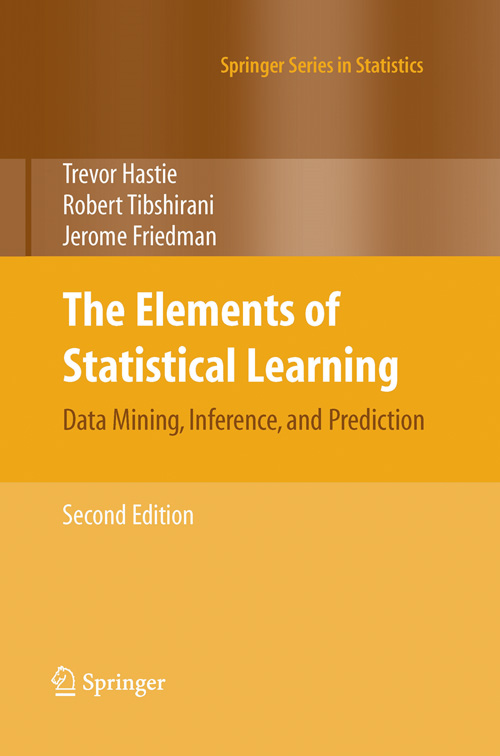
\includegraphics[width=0.20\textwidth]{books/ESLII.jpg}}
        \subfigure[]{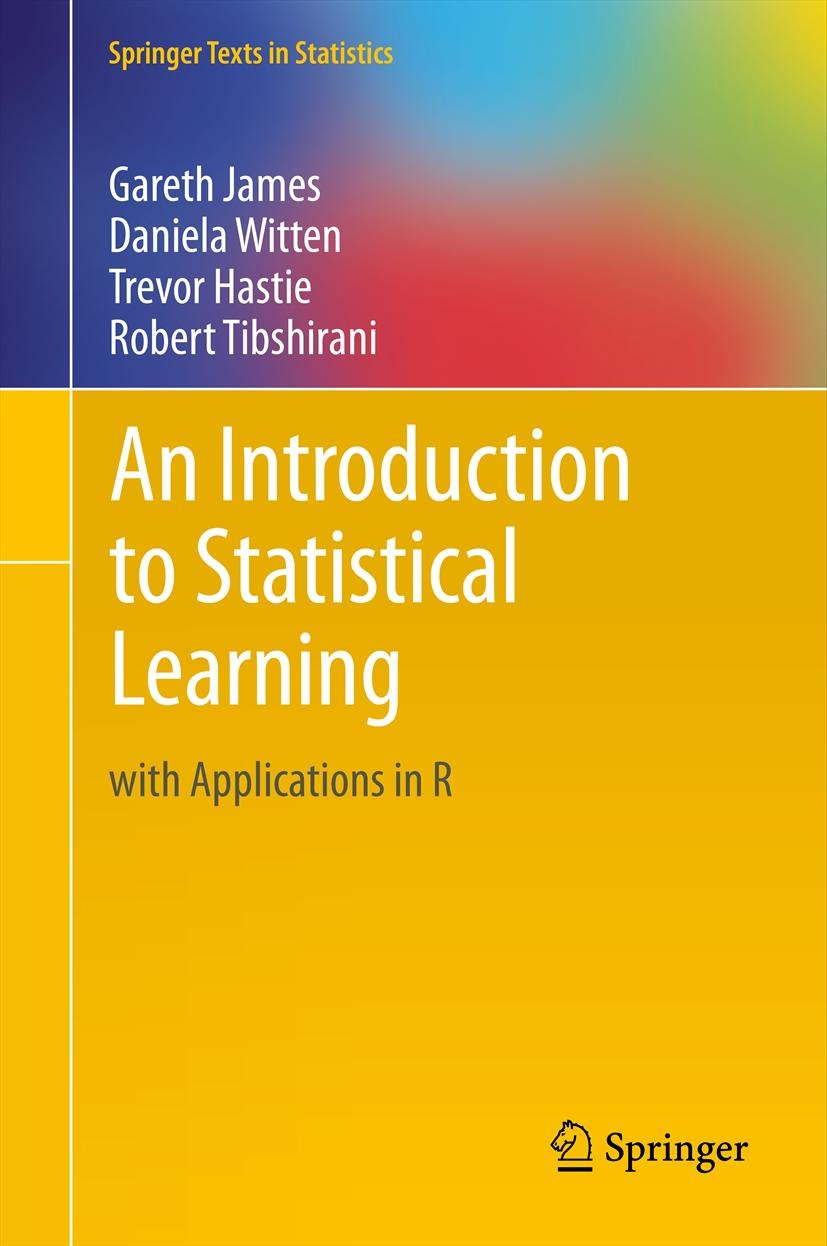
\includegraphics[width=0.20\textwidth]{books/ISL_Cover_2.jpg}} 
        \subfigure[]{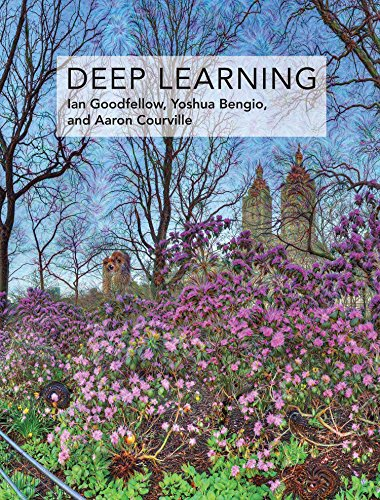
\includegraphics[width=0.20\textwidth]{books/DeepL.jpg}}
        \subfigure[]{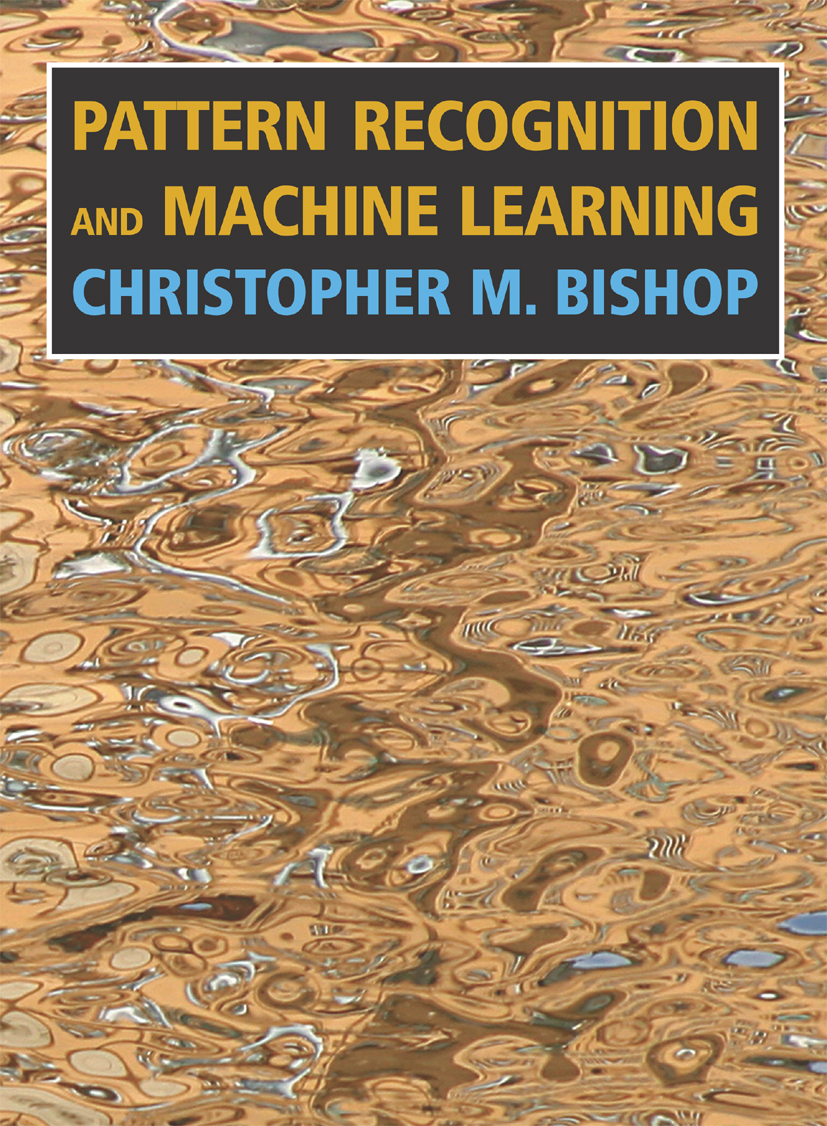
\includegraphics[width=0.20\textwidth]{books/Pattern.jpg}}
    \caption{(a) \href{https://web.stanford.edu/~hastie/ElemStatLearn/}{Elements of Statistical Learning} (b) \href{http://www-bcf.usc.edu/~gareth/ISL/}{Introduction to Statistical Learning} (c) \href{http://www.deeplearningbook.org/}{Deep Learning} (d) \href{https://www.microsoft.com/en-us/research/people/cmbishop/\#!prml-book}{Pattern Recognition and Machine Learning}}
    \end{figure}
\end{frame}

\begin{frame}{Machine Learning vs. Statistical Learning}
    \begin{itemize}
        \item \bred{Machine Learning (ML)} surgi\'o como un subcampo de la Inteligencia Artificial.
        \item \bblue{Statistical Learning (SL)} surgi\'o como un subcampo de la Estad\'istica.
        \item \textbf{Existe mucho traslapo}, ya que ambos campos se concentran en problemas Supervisados y No Supervisados:
        \begin{itemize}
            \item ML se concentra m\'as en \bred{aplicaciones a gran escala} y en la \bred{precisi\'on de la predicci\'on}.
            \item SL se concentra m\'as en los \bblue{modelos}, su interpretabilidad, en la \bblue{precisi\'on} e \bblue{incertidumbre}.
        \end{itemize}
        \item \textit{\textbf{La distinci\'on es cada vez m\'as borrosa.}}
    \end{itemize}
\end{frame}


\begin{frame}{Introducci\'on: Una Visi\'on General de SL}
    \begin{itemize}
        \item \defi{Aprendizaje estad\'istico} se refiere a una serie de herramientas para entender datos.
        \item Podemos clasificar a dichas herramientas como \textbf{supervisadas} y \textbf{no supervisadas}.
        \begin{itemize}
            \item Tercera area: \textit{aprendizaje por refuerzo (RL)}, el cual no veremos.
        \end{itemize} 
    \end{itemize}
\end{frame}

\begin{frame}{Aprendizaje Supervisado (SL)}
    \begin{itemize}
        \item En el \defi{aprendizaje supervisado (SL)}, construimos un modelo estad\'istico para estimar un resultado medible $Y$ a partir de mediciones $X$.
        \item $Y$ tambi\'en es llamado la variable dependiente, \bblue{variable de respuesta}, \bred{variable de salida} o variable objetivo.
        \item $X$ es un vector de $p$ \bblue{mediciones predictoras}, tambi\'en llamadas \bred{variable de entrada}, regresores, covariables, caracter\'isticas o variables independientes.
        \item El objetivo de SL entonces es de predecir el valor de $Y$ dado $X$, con (bastantes) ejemplos o instancias de estas medidas:
        \[ \{(x_{1}, y_{1}), \cdots, (x_{n}, y_{n}) \} \]
    \end{itemize}
    
\end{frame}

\begin{frame}{SL - Tipos de variables}
\begin{itemize}
    \item Por lo tanto, $Y$ puede ser:
    \begin{itemize}
        \item \textbf{Discreta} (cualitativa o categ\'orica)
        \item \textbf{Continua} (cuantitativa)
        \item \textbf{Ordenada categ\'orica} (el \'orden es importante)
    \end{itemize}
    \item Si estamos prediciendo una variable discreta, nos referimos al problema como de \defi{clasificaci\'on}.
    \item Si estamos prediciendo una variable continua, nos referimos al problema como de \defi{regresi\'on}.
\end{itemize}
\end{frame}

\begin{frame}{Aprendizaje No Supervisado (UL)}
    \begin{itemize}
        \item En el \defi{aprendizaje no supervisado (UL)}, no tenemos variable de salida, solamente un conjunto de predictores (caracter\'isticas) medidos en un conjunto de muestras.
        \item El objetivo final est\'a m\'as difuso y depende de la aplicaci\'on: encontrar subgrupos (clusters), subconjunto de predictores que se comporten de igual manera, o bien una combinaci\'on lineal de \'estos que tengan la mayor variaci\'on.
        \item Puede ser \'util para preprocesamiento de datos a utilizar en SL.
        \item No hay una m\'etrica \textit{per se}, por lo que es dif\'icil medir qu\'e tan bien nos va.
    \end{itemize}
\end{frame}

\begin{frame}{Notaci\'on (1)}
    \begin{itemize}
        \item $n$ representar\'a el n\'umero de puntos de datos distintos u observaciones en nuestra muestra.
        \item $p$ denotar\'a el n\'umero de variables que tenemos para realizar predicciones. 
        \begin{itemize}
            \item En algunos casos, $p>n$ e inclusive $p\gg n$, lo cual es com\'un para muestras biol\'ogicas.
        \end{itemize}
        \item Sea $x_{ij}$ el valor de la variable $j$ para la observaci\'on $i$, donde $i=1,\cdots, n$ y $j=1,\cdots,p$. Esto quiere decir que podemos ordernar a nuestros datos en una forma matricial:
        
        $$ \matr{X} = \begin{pmatrix} 
                    x_{11} & x_{12} & \dots & x_{1p} \\
                    x_{21} & x_{22} & \dots & x_{2p} \\
                    \vdots & \vdots & \ddots & \vdots\\
                    x_{n1} & x_{n2} & \dots & x_{np}
        \end{pmatrix} $$
    \end{itemize}
\end{frame}

\begin{frame}{Notaci\'on (2)}
    \begin{itemize}
        \item Denotaremos a $x_i$ como el $i-$\'esimo valor observado de $X$, donde $x_{i}$ es un vector de longitud $p$, el cual contiene las mediciones de las $p$ variables para la observaci\'on $i$:
        $$ x_{i} = \begin{pmatrix}
                    x_{i1}\\
                    x_{i2}\\
                    \vdots\\
                    x_{ip}
                    \end{pmatrix}$$
        \item Las columnas de $\matr{X}$ ser\'an denotadas por $\matr{x}_{j}$, un vector de longitud $n$ que contiene los valores de la variable $j$ en los $n$ datos:
        $$ \matr{x}_{j} = \begin{pmatrix}
                    x_{1j}\\
                    x_{2j}\\
                    \vdots\\
                    x_{nj}
                    \end{pmatrix}$$
    \end{itemize}
\end{frame}

\begin{frame}{Notaci\'on (3)}
    \begin{itemize}
        \item Por lo tanto, podemos escribir a $\matr{X}$ de las siguientes maneras:
         \begin{center}$\matr{X} = \begin{pmatrix} x_{1}^\intercal \\ x_{2}^\intercal \\ \vdots \\ x_{n}^\intercal\end{pmatrix}\qquad$ \'o $\qquad\matr{X} = \begin{pmatrix} \matr{x}_1 & \matr{x}_2 & \dots & \matr{x}_p \end{pmatrix}$
         \end{center}
        \item $X$ denotar\'a una \defi{variable de entrada}.
        \item $Y$ denotar\'a una \defi{variable de salida cuantitativa} (continua).
        \item $G$ denotar\'a una \defi{variable de salida cualitativa} (discreta).
        \item Utilizaremos a $x_i$, $y_i$ y $g_i$, $i=1,\dots,n$ como los $i-$\'esimas instancias de $X$, $Y$ y $G$, respectivamente.
    \end{itemize}
\end{frame}

\begin{frame}{Notaci\'on (4)}
    \begin{itemize}
        \item $\mathcal{G}$ denotar\'a el conjunto que contiene todas las clases que $G$ puede tomar.
        \item Denotaremos a $\hat{Y}$ como la \textit{predicci\'on de salida} para un $X$ dado.
        \item Se presume que se tiene una \defi{serie de datos de entrenamiento etiquetados} para los problemas de regresi\'on:
        \[ \mathcal{T} =  \{(x_{1}, y_{1}), \cdots, (x_{n}, y_{n}) \} \]
        donde $x_i \in \mathbb{R}^p$ y $y_i\in\mathbb{R}$.
        \item Se presume que se tiene una \defi{serie de datos de entrenamiento etiquetados} para los problemas de clasificaci\'on:
        \[ \mathcal{T} =  \{(x_{1}, g_{1}), \cdots, (x_{n}, g_{n}) \} \]
        donde $x_i \in \mathbb{R}^p$ y $g_i\in\mathcal{G}$.
    \end{itemize}
\end{frame}


\begin{frame}{Ejemplo - SL}
    \begin{figure}\label{fig:ej_numeros}
    \centering
        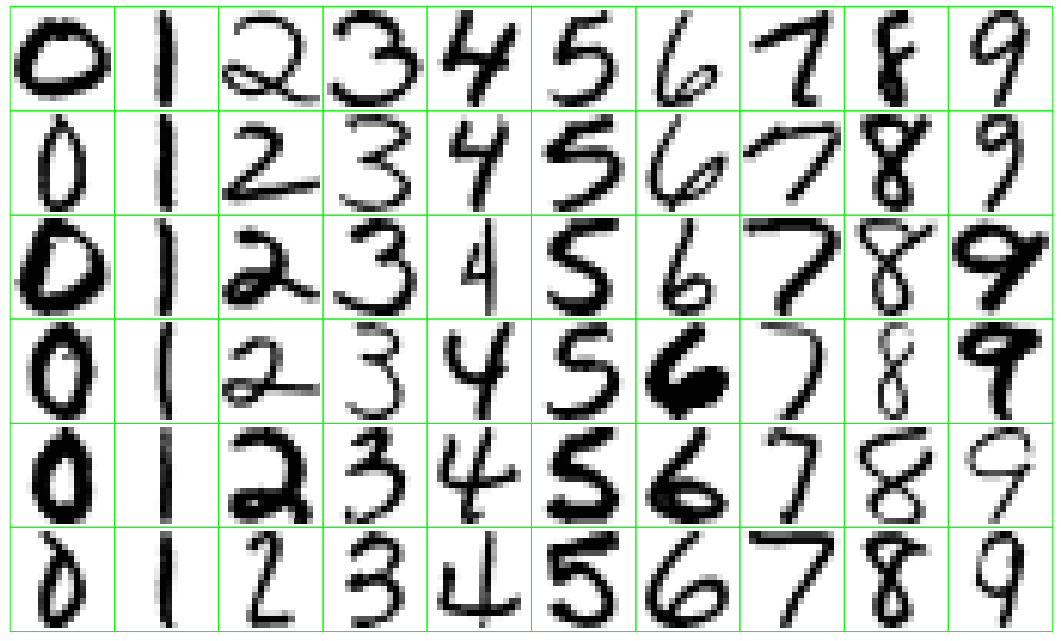
\includegraphics[width=0.70\textwidth]{images/esl/fig_1_2.PNG}
    \caption{Ejemplos de im\'agenes de digitos escritos a mano de sobres postales de los EE.UU. Cada imagen es de $16\times16$ pixeles de ocho bits, y cada pixel tiene una intensidad de 0 a 255. Por lo tanto, $\mathcal{G}=\{0,1,2,3,4,5,6,7,8,9\}$ y queremos clasificar correctamente cada imagen.}
    \end{figure}
\end{frame}

\begin{frame}{Ejemplo - UL}
    \begin{figure}\label{fig:ej_adn}
        \centering
        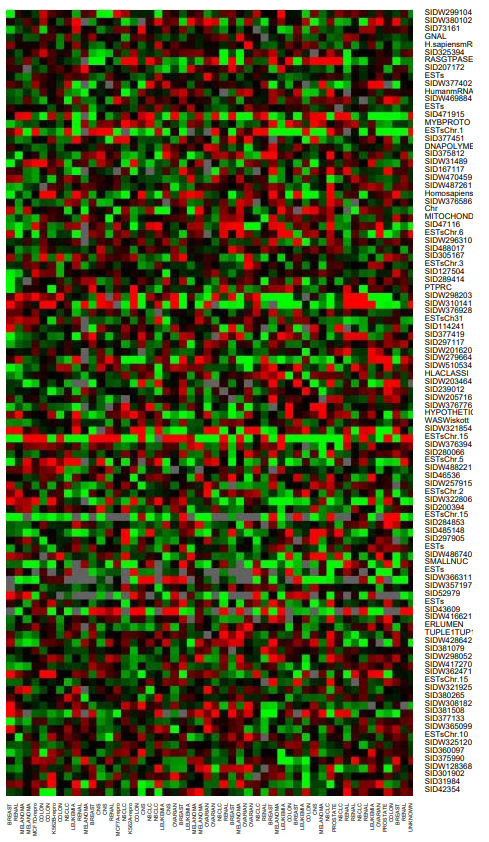
\includegraphics[width=0.40\textwidth, angle=270]{images/esl/fig_1_3.PNG}
        \caption{Datos de ADN: matriz de expresi\'on de $p=6830$ genes (columnas) y $n=64$ muestras (filas) de tumores de distintos pacientes. Se muestran 100 columnas \'unicamente (de manera aleatoria). Los valores van de verde claro (negativo) a rojo (positivo). Estamos interesados en si hay grupos o \textit{clusters}.}
    \end{figure}
\end{frame}

\begin{frame}{Una motivaci\'on (1)}
    \begin{itemize}
        \item Suponga que es lo contratan para analizar los datos de publicidad de una empresa.
        \item La empresa tiene datos de cu\'anto gasta en tres distintos medios \vari{TV}, \vari{radio} y \vari{peri\'odico}, as\'i como las $\vari{ventas}=Y$ en m\'as de $200$ mercados.
        \item Podemos asignar a $X_1$ al presupuesto asignado a \vari{TV}, $X_2$ al presupuesto asignado a \vari{radio} y $X_3$ al presupuesto asignado a \vari{peri\'odico} (aleatoriamente).
        \item Si la empresa desea establecer cu\'al medio es m\'as importante para invertir en publicidad e incrementar sus ventas, debemos de tomar a $X=(X_{1}, X_{2}, X_{3})$ y $Y$ (i.e., $\mathcal{T}$) y generar un \textbf{modelo}:
        
        \[ \vari{ventas} \approx f(\vari{TV}, \vari{radio}, \vari{peri\'odico})\]
    \end{itemize}
\end{frame}

\begin{frame}
\frametitle{Una motivaci\'on (2)}

\tikzstyle{na} = [baseline=-.5ex]

\begin{itemize}
    \item En otras palabras, asumimos que existe una relaci\'on del tipo:
        \begin{equation}\label{eq:1_funct}
            Y = f(X) + \epsilon
        \end{equation} 
        donde $X=(X_1, \dots, X_p)$ y $\epsilon$ es un \defi{t\'ermino de error} aleatorio (o \defi{error irreducible}), independiente de $X$ y con media $0$.
        \tikz[na] \node[coordinate] (n1) {};
        % Below we mix an ordinary equation with TikZ nodes. Note that we have to
% adjust the baseline of the nodes to get proper alignment with the rest of
% the equation.
\begin{equation*}
        \tikz[baseline]{
            \node[fill=blue!20,anchor=base] (t1)
            {$ \mathbb{E} \left[ \epsilon \right] = 0$};
        }
\end{equation*}

% Now it's time to draw some edges between the global nodes. Note that we
% have to apply the 'overlay' style.
\begin{tikzpicture}[overlay]
        \path[->]<1-> (n1) edge [bend left] (t1);

\end{tikzpicture}
        \item Desconocemos a $f$, por lo que debemos de \textit{estimarla} utilizando los datos observados.
\end{itemize}


\end{frame}

\begin{frame}{Una motivaci\'on (3)}
    \begin{itemize}
        \item ?`Para qu\'e queremos encontrar a $f$?
        \begin{itemize}
            \item Deseamos realizar \textbf{predicciones} de $Y$ cuando $X=x$:
            \begin{equation}\label{eq:1_pred}
                \hat{Y} = \hat{f}(X)
            \end{equation}
            \item Podremos entender cu\'ales componentes de $X=(X_1, \dots, X_p)$ son importantes para poder explicar a $Y$ (\textbf{inferencia}).
            \item Dependiendo de la complejidad de $f$, podremos entender qu\'e tanto afecta cada $X_j \in X$ a $Y$.
        \end{itemize}
        \item[$\star$] Por lo que, en esencia SL se refiere a un conjunto de m\'etodos para estimar a $f$.
    \end{itemize}
\end{frame}



\begin{frame}
\frametitle{Una motivaci\'on (4)}

\tikzstyle{na} = [baseline=-.5ex]

\begin{itemize}
    \item Si asumimos que tanto $\hat{f}$ y $X$ est\'an fijos, entonces (usando a las Ecuaciones \ref{eq:1_funct} y \ref{eq:1_pred}):

\begin{equation*}
\begin{aligned}
\mathbb{E}\left[ (Y - \hat{Y})^2\right] &= \mathbb{E}\left[ (f(X) + \epsilon - \hat{f}(X))^2 \right] \\
&= \mathbb{E}\left[ (f(X) - \hat{f}(X))^2 \right] + 2 \mathbb{E} \left[ (f(X) - \hat{f}(X)) \epsilon \right] + \mathbb{E}\left[\epsilon^2\right]\\
&= \mathbb{E}\left[ (f(X) - \hat{f}(X))^2 \right] + 2 \mathbb{E} \left[ f(X) - \hat{f}(X)\right] \mathbb{E} \left[\epsilon \right] + \\
& \qquad + \mathbb{E}\left[\left(\epsilon-0\right)^2\right]
\end{aligned}
\end{equation*}

    \item Es decir:
\begin{equation}\label{eq:1_errores}
    \mathbb{E}\left[ (Y - \hat{Y})^2\right] =\tikz[baseline]{
            \node[fill=blue!20,anchor=base] (t2)
            {$ (f(X) - \hat{f}(X))^2$};
        } +
        \tikz[baseline]{
            \node[fill=red!20,anchor=base] (t3)
            {$\mathbb{V}(\epsilon)$};
        }
\end{equation}

\begin{itemize}
    \item \textbf{Error reducible}
        \tikz[na]\node [coordinate] (n2) {};
    \item \textbf{Error irreducible}
        \tikz[na]\node [coordinate] (n3) {};
\end{itemize}

% Now it's time to draw some edges between the global nodes. Note that we
% have to apply the 'overlay' style.
\begin{tikzpicture}[overlay]
        \path[->]<3-> (n2) edge [bend right] (t2);
        \path[->]<4-> (n3) edge [out=0, in=-90] (t3);
\end{tikzpicture}
\end{itemize}
\end{frame}

\begin{frame}{?`C\'omo estimamos a $f$? (1)}
    \begin{itemize}
        \item Imaginen que tenemos una serie de datos:
        
        \begin{figure}
            \centering
            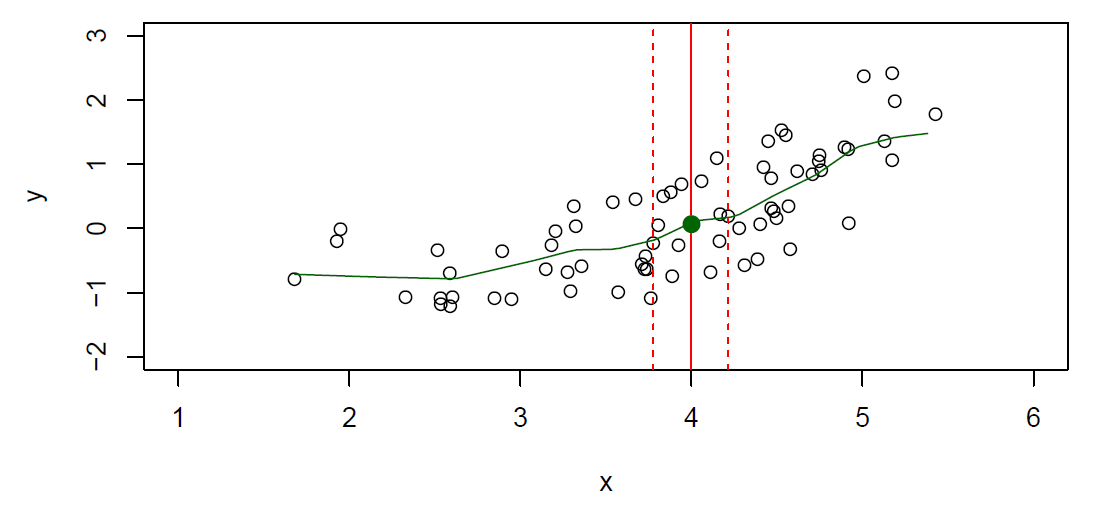
\includegraphics[width=0.60\textwidth]{images/v_esperado.PNG}
        \end{figure}
        
        \item $f(x)=\mathbb{E}\left[ Y \middle\vert X=x \right]$ ser\'a la \defi{funci\'on de regresi\'on}.
        \item ?`Cu\'al es un buen valor de $f(X)$ cuando $X=4$?
        \item No siempre podremos encontrar dicho valor, por lo que podemos \textit{relajar} la definici\'on:
        $$ \hat{f}(x) = \text{Ave}(Y \vert X \in \mathcal{N}(x)) $$
        
        donde $\mathcal{N}(x)$ es un \textit{vecindario} de $x$.
    \end{itemize}
\end{frame}

\begin{frame}{?`C\'omo estimamos a $f$? (2)}
    \begin{itemize}
        \item El promedio puede funcionar muy bien para $p \leq 4$ y un $n$ (mas o menos) grande.
        \item Todo se rompe en dimensiones altas (\textbf{maldici\'on de la dimensi\'on}).
        \item ?`Qu\'e proporci\'on de puntos se encuentran en la \textit{frontera} de un hipercubo unitario de dimensi\'on $d=50$?
        \begin{itemize}
            \item Nuestro hipercubo se define como $[0, 1]^d=[0,1]^{50}$. 
            \item La frontera se definir\'a como el conjunto de todos los puntos para el que existe un $j$ tal que $0\leq x_j \leq 0.05$ \'o $0.95 \leq x_j \leq 1$.
            \item Entonces, la proporci\'on de puntos que \textit{no} se encuentra en la frontera ser\'a:
            \[ \frac{(1-0.05-0.05)^{50}}{(1-0)^{50}} = \left(\frac{0.9}{1}\right)^{50} \approx 0.005 \]
            es decir, el $99.5\%$ de los puntos se encontrar\'a en la frontera.
        \end{itemize}
    \end{itemize}
\end{frame}

\begin{frame}{?`C\'omo estimamos a $f$? (3)}
    \begin{itemize}
        \item Si los datos est\'an repartidos uniformemente, vemos en graicado a la derecha a la longitud $a$ de la arista necesaria para que el subcubo capture una fracci\'on $r$ del volumen de datos: $a^p = r \iff a = r^{1/p}$.
        \begin{figure}
            \centering
            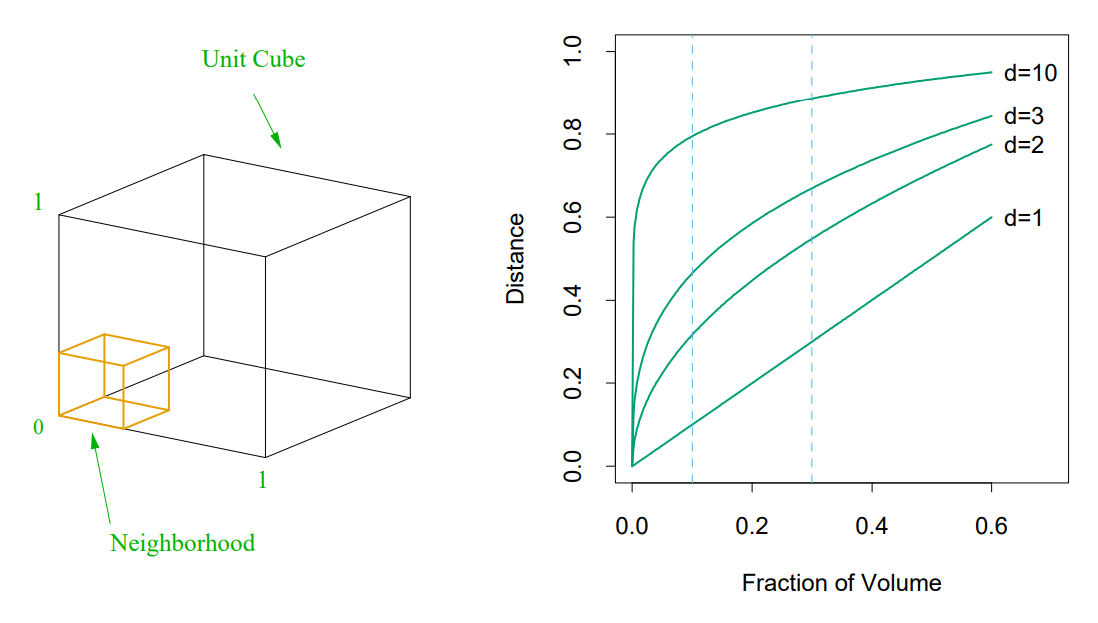
\includegraphics[width=0.45\textwidth]{images/esl/fig_2_6.PNG}
        \end{figure}
        \item Para $p=10$, para poder capturar $1\%$ de los datos ($r=0.01$), la arista esperada del subcubo medir\'a $a=0.01^{1/10}=0.63$, mientras que para capturar el $10\%$ de los datos, la arista del subcubo medir\'a $a=0.1^{1/10}=0.80$.
        \item El estimado del vecindario $\mathcal{N}(x)$ o \defi{vecinos cercanos} para $x$ \textbf{ya no ser\'a un m\'etodo local}.
    \end{itemize}
\end{frame}

\begin{frame}{Modelos Param\'etricos: Modelo Lineal (1)}
    \begin{itemize}
        \item Empezemos por el modelo param\'etrico m\'as sencillo (pero no necesariamente el m\'as simple): un \defi{model lineal}.
        \item Un modelo lineal predice el \textit{output} $Y$ de la siguiente manera:
        \begin{equation}\label{eq:1_modelo_lineal} \hat{Y} = \hat{\beta}_{0} + \sum_{j=1}^{p}X_{j}\hat{\beta}_{j} \end{equation}
        donde $\hat{\beta}_{0}$ es el \bblue{intercepto} o \bred{sesgo}.
        \item Un modelo lineal es especificado en t\'erminos de sus $p+1$ par\'ametros $\hat{\beta}_0, \dots, \hat{\beta}_p$.
    \end{itemize}
\end{frame}

\begin{frame}{Modelos Param\'etricos: Modelo Lineal (2)}
    \begin{itemize}
        \item Si bien casi nunca es acertado, el modelo lineal nos sirve para tener una aproximaci\'on interpretable de $f$.
        \item Si $X=(1, X_1, \dots, X_p)^\intercal$ y $\hat{\beta} = (\hat{\beta}_0, \dots, \hat{\beta_p})^\intercal$, entonces podemos escribir a la Ecuaci\'on \ref{eq:1_modelo_lineal} como:
        \begin{equation}
            \hat{Y} = X^\intercal \hat{\beta}
        \end{equation} 
        \item Estimamos a los par\'ametros al ajustar a nuestro modelo a los datos de entrenamiento $\mathcal{T}$.
        \item La forma m\'as com\'un es utilizando \textbf{m\'inimos cuadrados} para as\'i escoger a $\hat{\beta}$ que minimize la \defi{suma residual de cuadrados (RSS)}:
        \[ \text{RSS}(\beta) = \sum_{i=1}^{n} \left( y_i - x_{i}^{\intercal} \beta \right)^2 \]
    \end{itemize}
\end{frame}

\begin{frame}{Modelos Param\'etricos: Modelo Lineal (3)}
    \begin{itemize}
        \item Como RSS es una funci\'on cuadr\'atica, existir\'a un m\'inimo mas puede no ser \'unico.
        \item En notaci\'on matricial, podemos reescribir a RSS como:
        \begin{equation}\label{eq:1_rss}
        \text{RSS}(\beta) = (\matr{y} - \matr{X}\beta)^\intercal (\matr{y} - \matr{X}\beta)  \end{equation}
        donde $\matr{X}\in\mathbb{R}^{n\times (p+1)}$ y $\matr{y}\in \mathbb{R}^n$. 
        \item Si $\matr{X}^\intercal \matr{X}$ es no singular (tiene inversa), entonces la soluci\'on a 
        
        \[\hat{\beta} = \argmin_{\beta} (\matr{y} - \matr{X}\beta)^\intercal (\matr{y} - \matr{X}\beta)  \]
        
        esta dada por
        
        \begin{equation}\label{eq:1_normaleq} \hat{\beta} = (\matr{X}^\intercal \matr{X})^{-1} \matr{X}^\intercal \matr{y} \end{equation}
    \end{itemize}
\end{frame}

\begin{frame}{Modelos Param\'etricos: Modelo Lineal (4)}
	\begin{itemize}
		\item La ecuaci\'on \ref{eq:1_normaleq} se llama la \defi{ecuaci\'on normal} $\Rightarrow p+1$ par\'ametros .
		\item Se encuentra f\'acilmente al derivar a RSS respecto de $\beta$.
		\item Podemos encontrar num\'ericamente a $\hat{\beta}$ mediante la ecuaci\'on normal o utilizando el algoritmo de \textbf{descenso gradiente}.
		
		\begin{table}[bt]
			\begin{tabular}{|l|l|} \hline
				\textbf{Descenso Gradiente} & \textbf{Ecuaci\'on Normal} \\ \hline
				Necesitamos escoger $\alpha$ & No necesitamos escoger $\alpha$ \\
				Necesita muchas iteraciones  & No hay necesidad de iteraci\'on \\
				$\mathcal{O}(k p^2)$ & $\mathcal{O}(p^3)$\\
				Funciona bien aunque $p$ sea grande  & Lento cuando $p$ es grande\\ 
				\hline
			\end{tabular}
		\end{table}
		
	\end{itemize}
\end{frame}

\begin{frame}{Modelos Param\'etricos: Modelo Lineal (5)}
	\begin{itemize}
		\item ?`Qu\'e pasa si aplicamos el modelo de regresi\'on lineal a un conjunto de datos categ\'oricos?
		\item $\mathcal{T}=\{(x_i, y_i) \}_{i=1}^{n}$, con $y_i \in \{\textcolor{orange} {\mathtt{NARANJA}},\textcolor{Cerulean}{\mathtt{AZUL}}\}$.
		\item Un modelo de regresi\'on lineal nos dar\'a a $\hat{\beta}$ tal que:
		
		\begin{equation*} \hat{G} = \begin{cases}
		\textcolor{orange}{\mathtt{NARANJA}} & \text{si } X^\intercal \hat{\beta} > 0.5\\
		\textcolor{Cerulean}{\mathtt{AZUL}} & \text{si } X^\intercal \hat{\beta} \leq 0.5 \end{cases}  \end{equation*}
		
	\end{itemize}
\end{frame}

\begin{frame}{Modelos Param\'etricos: Modelo Lineal (6)}

\begin{figure}\label{fig:1_lineal_2clases}
	\centering
	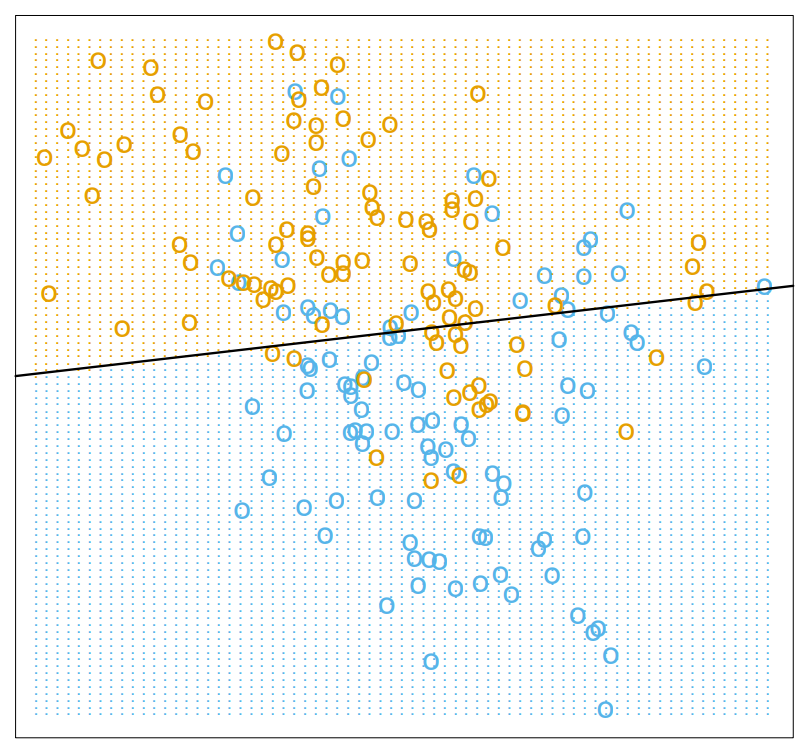
\includegraphics[width=0.4\textwidth]{images/esl/fig_2_1.PNG}
	\caption{Generamos datos en dos dimensiones con clases $\textcolor{Cerulean}{\mathtt{AZUL}}$ y $\textcolor{orange}{\mathtt{NARANJA}}$. Para realizar el modelo, codificamos a las clases como una variable binaria ($\textcolor{Cerulean}{\mathtt{AZUL}}=0$ y $\textcolor{orange}{\mathtt{NARANJA}}=1$). Vemos que el modelo lineal es demasiado r\'igido y, por inspecci\'on visual, las dos clases no son linealmente separables. $X^\intercal \hat{\beta} = 0.5$ define a la \textit{frontera de decisi\'on}.}
\end{figure}

\end{frame}

\begin{frame}{Modelos No Param\'etricos: Vecinos M\'as Cercanos (1)}
\begin{itemize}
	\item Definimos al modelo de \defi{k vecinos m\'as cercanos (KNN)} como:
	
	\begin{equation}\label{eq:1_knn}
		\hat{Y}(x) = \frac{1}{k} \sum_{x_i \in N_{k}(x)}y_i
	\end{equation}
	o en palabras: encuentre las $k$ observaciones $x_i$ m\'as cercanas a $x$ y calcule el promedio de sus respectivas respuestas $y_i$.
	\item ?`C\'omo definimos \textit{cercano}?
	\begin{itemize}
		\item Usaremos (en general) la \textbf{distancia Euclidiana} o \textbf{norma L2}. Para el vector $\matr{x} = (x_1, \dots , x_{p})$:
		\[ \lVert x_i\rVert_2 = \sqrt{\sum_{i=1}^{p}x_{i}^2} \]
		\item Existen m\'as normas que iremos definiendo cuando sea pertinente.
	\end{itemize}
\end{itemize}
\end{frame}

\begin{frame}{Modelos No Param\'etricos: Vecinos M\'as Cercanos (2)}

\begin{itemize}
	\item $k$ es un \textbf{hiperpar\'ametro}.
	\item Los par\'ametros de los modelos no crecen conforme $\mathcal{T}$ crece.
	\item \textbf{Ventaja principal}: 
	\begin{itemize}
		\item No asumimos la forma de $f$, por lo que cubren una mayor cantidad de formas de $f$.
	\end{itemize} 
	\item \textbf{Desventaja principal}:
	\begin{itemize}
		\item Necesitamos m\'as datos para conseguir un estimado correcto de $f$.
	\end{itemize}
\end{itemize}
\end{frame}


\begin{frame}{Modelos No Param\'etricos: Vecinos M\'as Cercanos (3)}
\begin{itemize}
	\item Para la clasificaci\'on binaria, $\mathcal{T}=\{(x_i,y_i)\}_{i=1}^{n}$, donde $g_i \in {0,1}$ (de regreso a nuestro ejemplo anterior.)
	\item El estimado de $G$, $\hat{G}$ dado por KNN es:
	
	\begin{equation*} \hat{G} = \begin{cases}
	\textcolor{orange}{\mathtt{NARANJA}} & \text{si } \frac{1}{k} \sum_{x_i \in N_k (x)} g_i > 0.5\\
	\textcolor{Cerulean}{\mathtt{AZUL}} & \text{si } \frac{1}{k} \sum_{x_i \in N_k (x)} g_i \leq 0.5 \end{cases}  
	\end{equation*}
	\item Es decir, encontramos las $k$ observaciones $x_i$ m\'as cercanas a $x$ y estimamos la clase de $x$ como la que pertenece la \textit{mayor\'ia} de sus vecinos.
\end{itemize}
\end{frame}

\begin{frame}{KNN, $k=15$}
	\begin{figure}\label{fig:1_knn15}
		\centering
		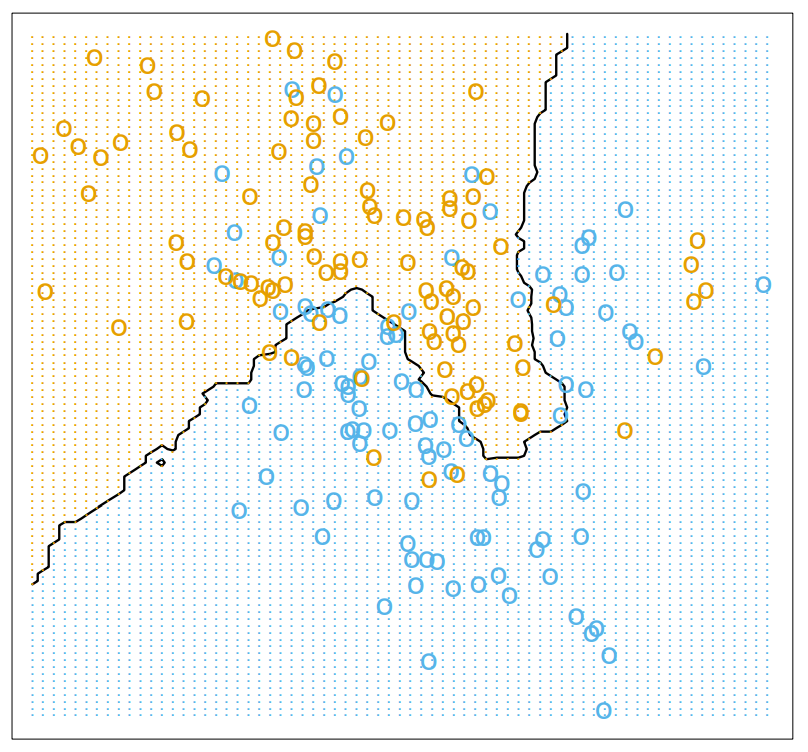
\includegraphics[width=0.5\textwidth]{images/esl/fig_2_2.PNG}
		\caption{Usamos los mismos datos que en la Figura \ref{fig:1_lineal_2clases}; codificamos a las clases como una variable binaria ($\textcolor{Cerulean}{\mathtt{AZUL}}=0$ y $\textcolor{orange}{\mathtt{NARANJA}}=1$) y lo ajustamos a un modelo de KNN con $k=15$. Por ende, la clase predicha es escogida por voto mayoritario entre los 15 vecinos m\'as cercanos.}
	\end{figure}
\end{frame}

\begin{frame}{KNN, $k=1$}
\begin{figure}\label{fig:1_knn1}
	\centering
	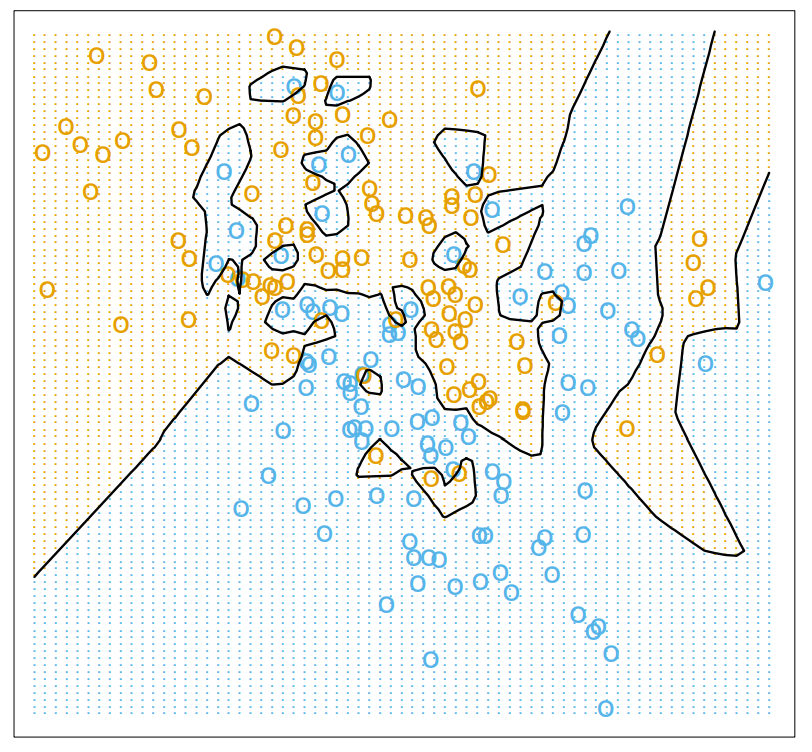
\includegraphics[width=0.5\textwidth]{images/esl/fig_2_3.PNG}
	\caption{Usamos los mismos datos que en la Figura \ref{fig:1_lineal_2clases}; codificamos a las clases como una variable binaria ($\textcolor{Cerulean}{\mathtt{AZUL}}=0$ y $\textcolor{orange}{\mathtt{NARANJA}}=1$) y lo ajustamos a un modelo de KNN con $k=1$. Llegamos a lo que comunmente se denomina como \defi{Teselaci\'on de Voronoi}.}
\end{figure}
\end{frame}

\begin{frame}{KNN}
\begin{itemize}
	\item N\'otese que para $k=1$, nuestro clasificador no comete errores.
	\item ?`Qu\'e tan bien le ir\'a clasificando datos que no ha visto antes?
	\item Definimos al \defi{conjunto de entrenamiento} $\mathcal{T}_{\text{Tr}}$ como los datos que utilizamos para entrenar nuestro algoritmos.
	\item Definimos a \defi{conjunto de prueba} $\mathcal{T}_{\text{Te}}$ como los datos que utilizamos para realizar predicciones utilizando a nuestro algoritmo.
	\item Es importante que no hayan datos cruzados, ni que se escogan a mano cu\'al ir\'a en cada conjunto.
	\begin{itemize}
		\item Para $\lvert\mathcal{T}\rvert \sim 100000$, $\lvert \mathcal{T}_{\text{Tr}} \rvert / \lvert \mathcal{T} \rvert \approx 0.7 $ y $\lvert \mathcal{T}_{\text{Te}} \rvert / \lvert \mathcal{T} \rvert \approx 0.3 $.
		\item Para $\lvert\mathcal{T}\rvert > 1000000$, $\lvert \mathcal{T}_{\text{Tr}} \rvert / \lvert \mathcal{T} \rvert \approx 0.98 $ y $\lvert \mathcal{T}_{\text{Te}} \rvert / \lvert \mathcal{T} \rvert \approx 0.02 $.
	\end{itemize}
\end{itemize}
\end{frame}

\begin{frame}[fragile]
\begin{semiverbatim}
\textcolor{deepblue}{import} numpy as np
\textcolor{deepblue}{from} sklearn.model\_selection \textcolor{deepblue}{import} train\_test\_split

X = np.random.randn(10).reshape((5, 2))

y = np.random.choice(2, 5)

X\_train, X\_test, y\_train, y\_test = train\_test\_split(
X, y, test\_size=0.3, random\_state=42, shuffle=True)
\end{semiverbatim}
\end{frame}

\begin{frame}{?`Qu\'e modelo elegimos?}
	\begin{itemize}
		\item Debemos de escoger una m\'etrica con la cual medir a nuestros modelos que hemos entrenado con el conjunto de entrenamiento $\mathcal{T}_{\text{Tr}}$.
		\item Espec\'ificamente, nos interesa saber qu\'e tan precisos son nuestros modelos tanto en $\mathcal{T}_{\text{Tr}}$ como en $\mathcal{T}_{\text{Te}}$.
		\item El \defi{error cuadr\'atico medio (MSE) de entrenamiento} es:
		\begin{equation}\label{eq:1_trainmse}
		\text{MSE}_{\mathcal{T}_{\text{Tr}}} = \text{Ave}_{i \in \mathcal{T}_{\text{Tr}}}(y_i - \hat{f}(x_i))^2
		\end{equation}
		\item El \defi{error cuadr\'atico medio (MSE) de prueba} calculado sobre $\mathcal{T}_{\text{Te}}$ es:
		\begin{equation}\label{eq:1_testmse}
		\text{MSE}_{\mathcal{T}_{\text{Te}}} = \text{Ave}_{i \in \mathcal{T}_{\text{Te}}}(y_i - \hat{f}(x_i))^2
		\end{equation}
	\end{itemize}
\end{frame}

\begin{frame}{Eligiendo a $k$ en KNN}
\begin{figure}\label{fig:1_errorKNN}
	\centering
	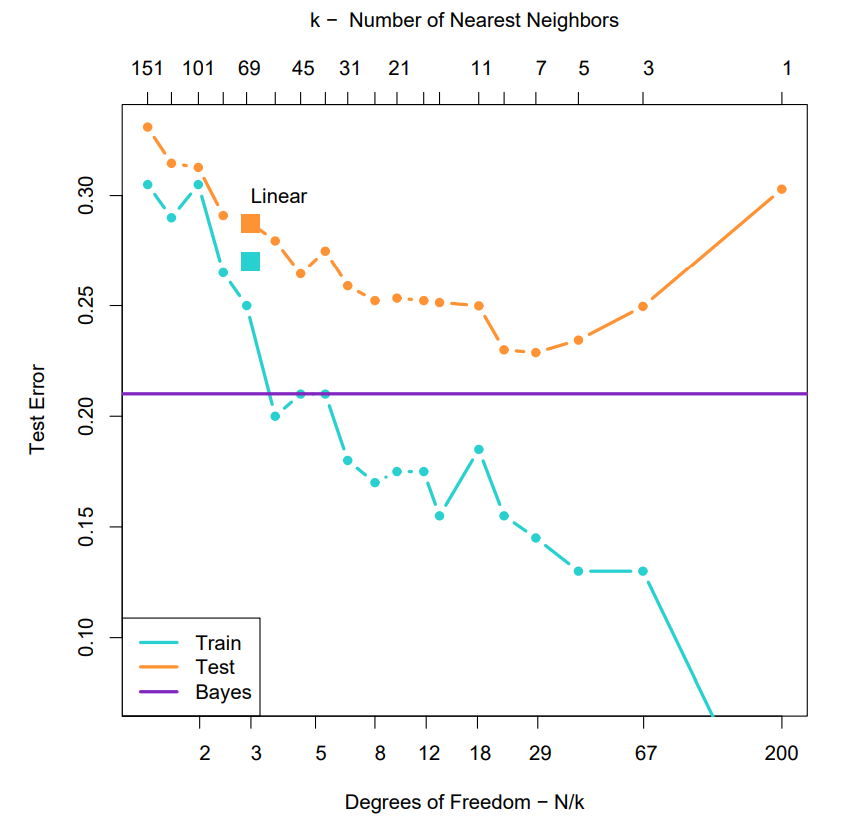
\includegraphics[width=0.45\textwidth]{images/esl/fig_2_4.PNG}
	\caption{Curvas de MSE de entrenamiento y de prueba para distintos valores de $k$. Se presentan adem\'as los mismos valores para nuestro modelo lineal. El error para la frontera de decisi\'on \'optima se conoce como el \defi{ritmo de error de Bayes}.}
\end{figure}

\end{frame}

\begin{frame}{Frontera de Decisi\'on de Bayes}
\begin{figure}\label{fig:1_fronterabayes}
	\centering
	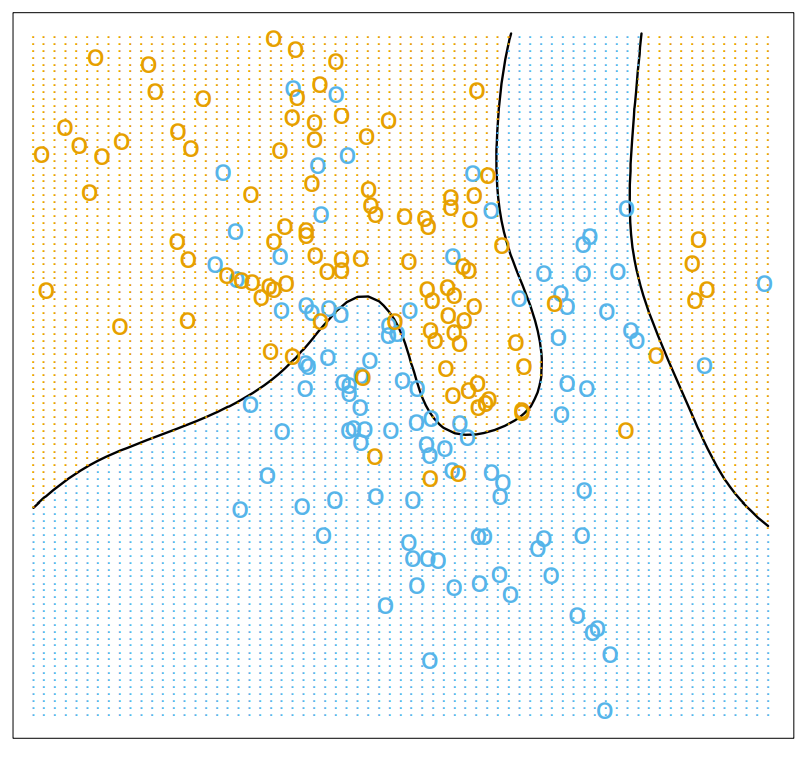
\includegraphics[width=0.5\textwidth]{images/esl/fig_2_5.PNG}
	\caption{La frontera de decisi\'on \'optima para los datos anteriores. La podemos calcular ya que se conocen las densidades de probabilidad para con las cuales se generaron las dos series de datos.}
\end{figure}

\end{frame}

\begin{frame}{MSE para Tres Curvas (1)}
\begin{figure}
	\centering
	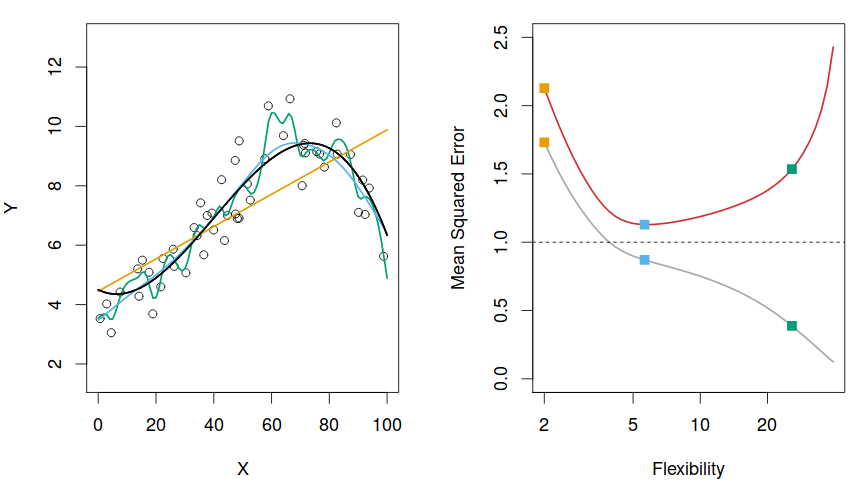
\includegraphics[width=0.7\textwidth]{images/islr/fig_2_9.png}
	\caption{La curva negra indica la funci\'on \textit{real} $f$ con la cual generamos los datos. Se muestran tres aproximaciones y sus respectivos $\text{MSE}_{\mathcal{T}_{\text{Tr}}}$ (en \textcolor{gray}{gris}) y $\text{MSE}_{\mathcal{T}_{\text{Te}}}$ (en \textcolor{red}{rojo}): regresi\'on lineal en naranja y dos \textit{curvas spline} en azul y verde. La l\'inea punteada representa el error de Bayes o $\mathbb{V}[\epsilon]$.}
	\label{fig:1_3curvas_1}
\end{figure}
\end{frame}

\begin{frame}{MSE para Tres Curvas (2)}
\begin{figure}
	\centering
	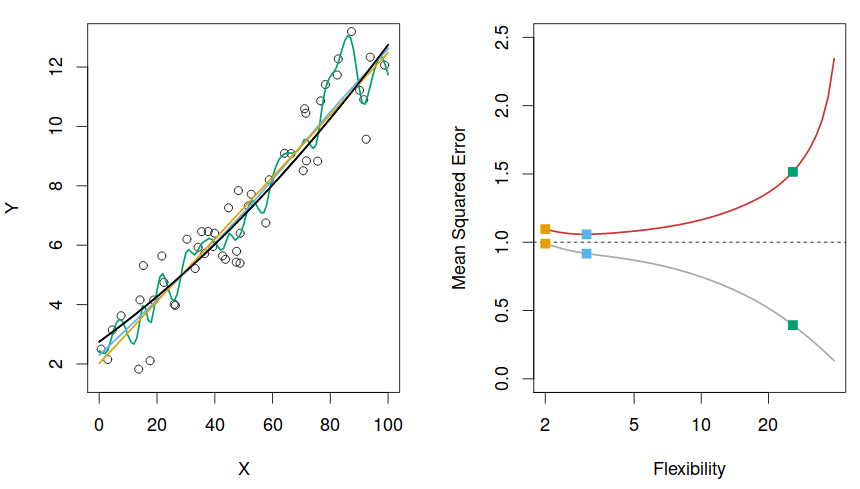
\includegraphics[width=0.7\textwidth]{images/islr/fig_2_10.png}
	\caption{Los detalles son los mismos que para la Figura \ref{fig:1_3curvas_1}. N\'otese que ya que $f$ es m\'as cercano  a ser lineal, la regresi\'on lineal realizar\'a un buen ajuste a los datos.}
	\label{fig:1_3curvas_2}
\end{figure}
\end{frame}

\begin{frame}{MSE para Tres Curvas (3)}
\begin{figure}
	\centering
	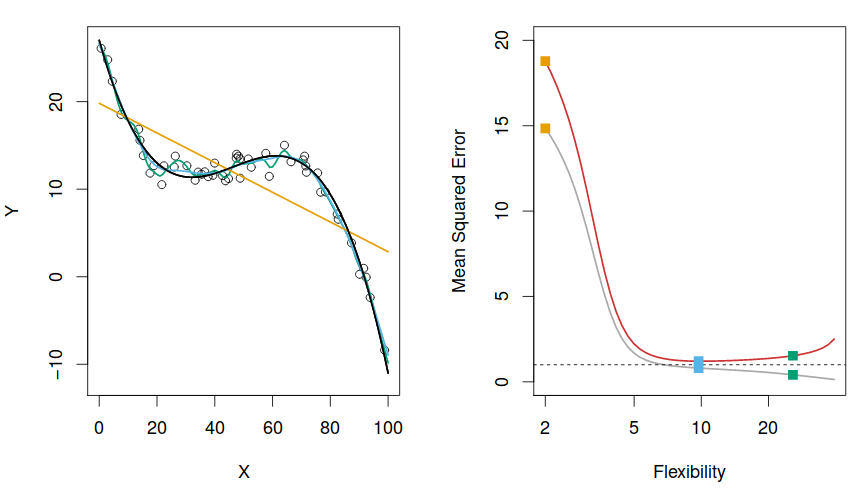
\includegraphics[width=0.7\textwidth]{images/islr/fig_2_11.png}
	\caption{Los detalles son los mismos que para la Figura \ref{fig:1_3curvas_1}. Ahora $f$ est\'a lejos de ser lineal, por lo que la regresi\'on lineal realizar\'a un ajuste muy pobre a los datos.}
	\label{fig:1_3curvas_3}
\end{figure}
\end{frame}

\begin{frame}{Intercambio entre Varianza y Sesgo (1)}
	\begin{itemize}
		\item Hacemos la siguiente observaci\'on:
		\begin{itemize}
			\item Mientras m\'as flexible sea un modelo, menor ser\'a su $\text{MSE}_{\mathcal{T}_{\text{Tr}}}$, pero mayor ser\'a su $\text{MSE}_{\mathcal{T}_{\text{Te}}}$.
			\item Por lo tanto, un $\text{MSE}_{\mathcal{T}_{\text{Tr}}}$ bajo \textbf{no es un buen indicador} de un $\text{MSE}_{\mathcal{T}_{\text{Te}}}$ bajo.
		\end{itemize}
	\item En general, podemos descomponer al $\text{MSE}_{\mathcal{T}_{\text{Te}}}$ de la siguiente manera para una observaci\'on de prueba $(x_0, y_0)$:
	
	\begin{align}
		\text{MSE}_{\mathcal{T}_{\text{Te}}}(x_0)&=\mathbb{E}_{\mathcal{T}_{\text{Te}}}[(y_0 - \hat{f}(x_0))^2]\\
		&= (\text{Bias}[\hat{f}(x_0)])^2 + \mathbb{V}[\hat{f}(x_0)] + \mathbb{V}[\epsilon]
	\end{align}
	donde \[\text{Bias}[\hat{f}(x)]=\mathbb{E}_{\mathcal{T}_{\text{Te}}}[\hat{f}(x)] - f(x) \qquad \mathbb{V}[\hat{f}(x)] = \mathbb{E}_{\mathcal{T}_{\text{Te}}}[\hat{f}(x)^2] - \mathbb{E}_{\mathcal{T}_{\text{Te}}}[\hat{f}(x)]^2 \]
	\end{itemize}
\end{frame}

\begin{frame}{Intercambio entre Varianza y Sesgo (2)}
\begin{itemize}
	\item Queremos entonces que nuestra estimaci\'on $\hat{f}$ obtenga un sesgo (Bias) bajo y una varianza baja.
	\item Error irreducible :(
	\item \defi{Varianza} de un modelo se refiere a la cantidad que $\hat{f}$ cambiar\'ia si usaramos un conjunto de entrenamiento distinto para ajustarlo.
	\item \defi{Bias} (o \defi{Sesgo}) se refiere al error introducido al tratar de aproximar un problema de la vida real.
	\item El \defi{intercambio entre varianza y sesgo} se refiere al hecho de que los modelos con sesgo bajo tienen varianza alta y viceversa $\Rightarrow$ \textbf{dilemma}.
\end{itemize}
\end{frame}

\begin{frame}{Intercambio entre Varianza y Sesgo (3)}
\begin{figure}
	\centering
	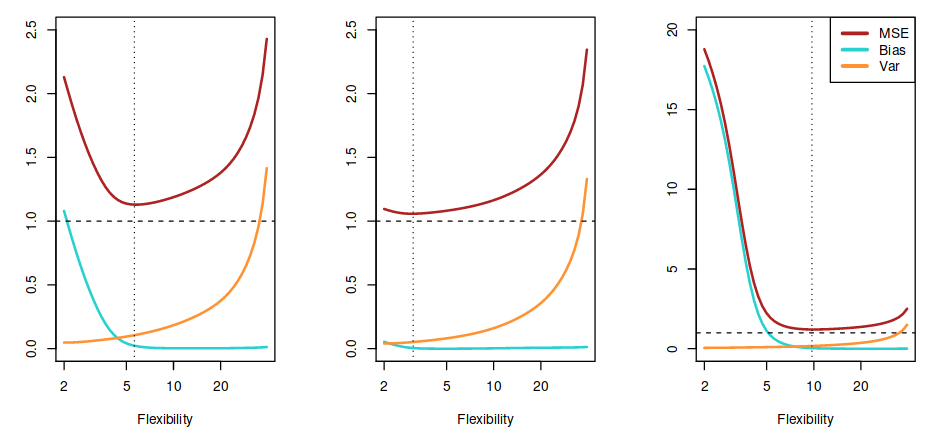
\includegraphics[width=0.7\textwidth]{images/islr/fig_2_12.png}
	\caption{Descomposici\'on del $\text{MSE}_{\mathcal{T}_{\text{Te}}}$ para los datos de las Figuras \ref{fig:1_3curvas_1}, \ref{fig:1_3curvas_2} y \ref{fig:1_3curvas_3}. La l\'inea vertical punteada indica el nivel de flexibilidad correspondiente al valor m\'inimo de $\text{MSE}_{\mathcal{T}_{\text{Te}}}$. En problemas reales, solo tendremos que estimar a $\text{MSE}_{\mathcal{T}_{\text{Te}}}$, usando, por ejemplo, \textbf{validaci\'on cruzada}.}
	\label{fig:1_int_b_var}
\end{figure}
\end{frame}

\begin{frame}{Intercambio entre Varianza y Sesgo (4)}
\begin{figure}
	\centering
	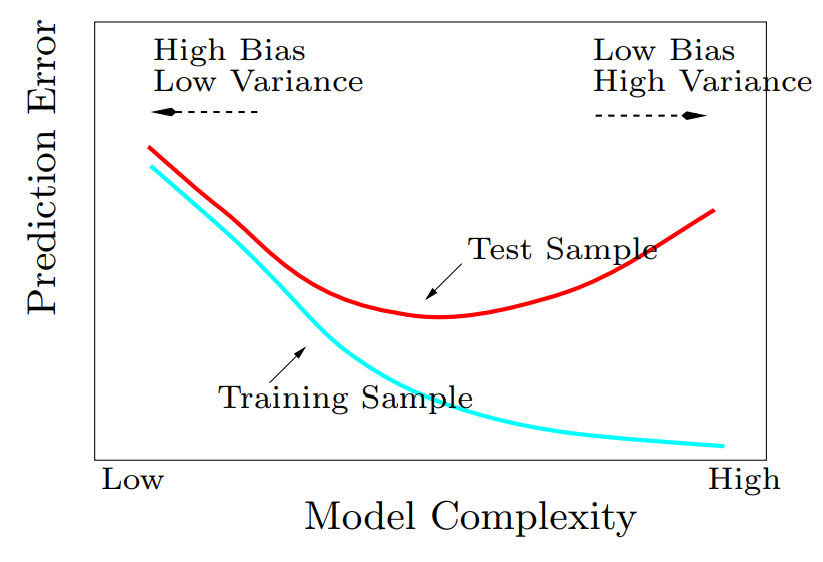
\includegraphics[width=0.7\textwidth]{images/esl/fig_2_11.PNG}
	\caption{ $\text{MSE}_{\mathcal{T}_{\text{Te}}}$ y $\text{MSE}_{\mathcal{T}_{\text{Tr}}}$ en funci\'on de la complejidad del modelo. Si tenemos Bias alto y Varianza baja, tenemos un problema de \defi{underfitting}. Si tenemos el Bias bajo y la Varianza alta, tenemos un problema de \defi{overfitting}.}
	\label{fig:1_over_under}
\end{figure}
\end{frame}

\begin{frame}{Intercambio entre Precisi\'on e Interpretabilidad}
\begin{figure}\label{fig:1_flexi}
	\centering
	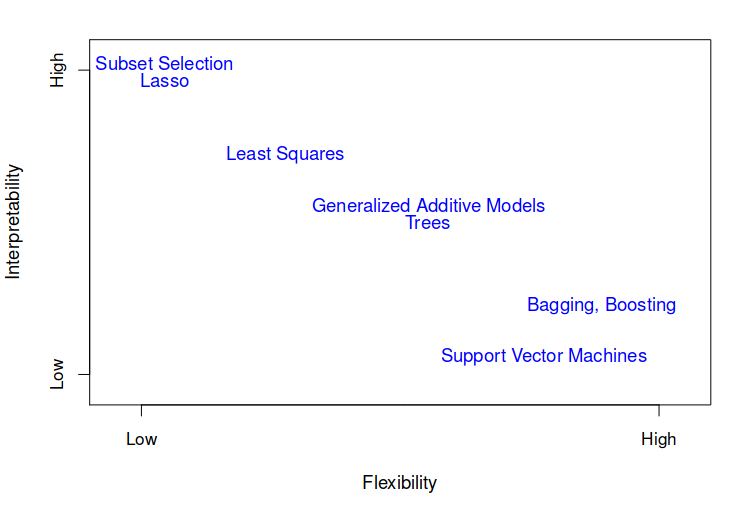
\includegraphics[width=0.6\textwidth]{images/islr/fig_2_7.png}
\end{figure}
\begin{itemize}
	\item Mientras mas \defi{flexible} un modelo, ser\'a mayor su capacidad de generar funciones para aproximar a $f$.
	\item Preferimos modelos mas simples que involucren menos variables sobre un predictor de \textbf{caja negra} que involucre todas las variables.
\end{itemize}
\end{frame}

\end{document}